%%=============================================================================
%% Voorgeschiedenis Universiteit Gent
%%=============================================================================

\chapter{Voorgeschiedenis van het netwerk van Universiteit Gent}%
\label{ch:voorgeschiedenis}
Dit hoofdstuk wordt eerst een overzicht gegeven van de huidige werking voor netwerkbeheerders binnen UGent.
Daarna wordt beschreven welke stappen reeds zijn ondernomen om deze werking aan te passen om EfficientIP te implementeren.

\section{Huidige werking Universiteit Gent}
Bij de aanvang van de bachelorproef is het netwerk van UGent nog volledig beheerd via subnetbestanden. Binnen het netwerkteam van UGent werd een standaard bepaald en toegepast voor het nummeren en klasseren van subnetten, de zogenaamde ARWA-standaard (naar oud-werknemer ARsene WAuters). Dankzij scripts worden deze subnetbestanden uitgelezen en wordt alle nodige informatie doorgegeven aan o.a. de DNS- en DHCP-servers. Daarnaast genereren deze scripts ook \acrfull{acl}-regels die dan via update-scripts op de routers kunnen geplaatst worden.

\subsection{Subnetbestanden}
\label{subnetbestanden}
Op basis van ARWA-standaard krijgt elk subnetbestand een naam: “subnet” + subnet klasse (A/B/C/D/G/I/N/P/T/V/W) + subnetnummer (laatste 2 octetten van het netwerkadres). Elk subnetwerk binnen UGent komt overeen met een of meerdere subnetbestanden, afhankelijk van de grootte van het subnetwerk. Een subnetwerk dat meer dan 254 beschikbare IP-adressen bevat, komt overeen met meerdere opeenvolgende subnetbestanden. Indien een subnetwerk minder dan 254 hostadressen bevat, bijvoorbeeld 126, zal dit subnetbestand ook maar 126 hosts bevatten.
Zo stelt bijvoorbeeld het subnetbestand “subnetB147.000” het subnet 157.193.147.0/24 voor, en subnetbestand “subnetB050.128” het subnet 157.193.50.128/25. Deze ongecrypteerde tekstbestanden stellen elk een deel, of een volledig subnet voor. Elk subnetbestand bestaat telkens uit twee delen: 
\begin{itemize}
    \item \textbf{Header}: Elk bestand begint met een “header” waarin belangrijke metadata beschreven staat over het netwerk, een voorbeeld is terug te vinden in figuur \ref{fig:header}. Belangrijk om hier nog te vermelden is dat het metadataveld 'subnet plaats' de gebouwcodes (FI-codes) opsomt die door de Universiteit Gent \\(UGent) worden gebruikt om aan te geven waar dit subnet actief is. Dit is relevant om te weten aangezien dit gebruikt kan worden om een verband te leggen tussen subnetten en gebouwen. Daarnaast staan de optionele S-lijnen voor \acrfull{acl}-lijnen (beveiligingregels die toegang geven of weigeren voor een of meerdere subnetten of hosts) om extra toegang te voorzien aan het netwerk. 
    \item \textbf{Hosts}: Afhankelijk van de grootte van het subnet kunnen er tot 254 hosts beschreven staan in het bestand. Elk hostadres, of die nu reeds bezet is of niet, staat beschreven in het subnetbestand. Hierbij krijg je dan een opsomming van alle informatie, waarbij elk informatieveld wordt voorafgegaan door de relevante code. Een hostadres dat niet bezet is, bevat naast het nummer (die het laatste octet weergeeft van het IP-adres) enkel lege velden, zoals te zien in \ref{fig:legehost}. Naast de data voor elke host kan een netwerkbeheerder ook extra lijnen toevoegen voor DNS, namelijk A en CNAME resource records “AA: en CA:”, de beveiliging richting de host met “S: en SI:” openzetten en ook extra mailinformatie “MD:” toevoegen. Een voorbeeld van een bezette host staat weergegeven in figuur \ref{fig:bezettehost}.
\end{itemize}

\begin{figure}[H]
    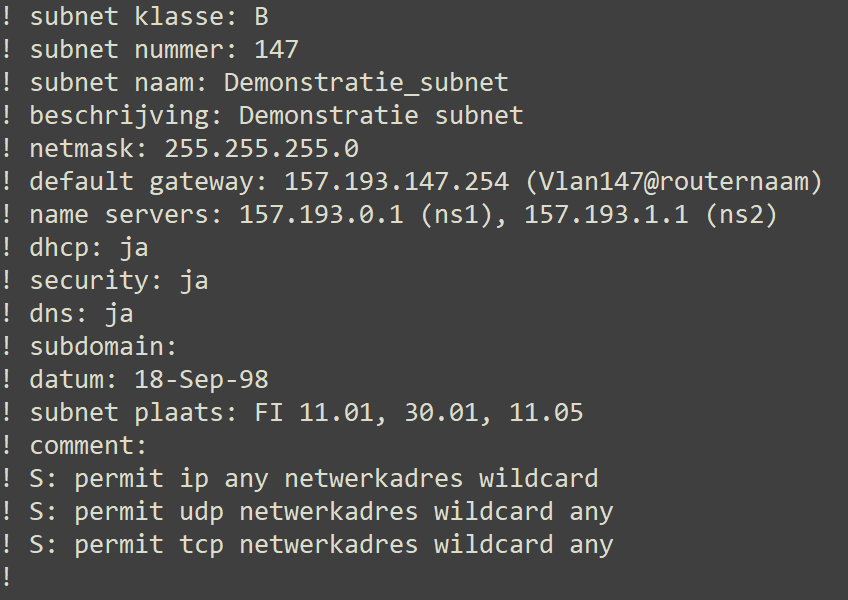
\includegraphics[height=7cm]{header.png}
    \caption{Header in subnetbestanden}
    \label{fig:header}
\end{figure}

\begin{figure}[H]
    \subfloat[IP-reservatie voor het eerste adres in het subnet]{%
        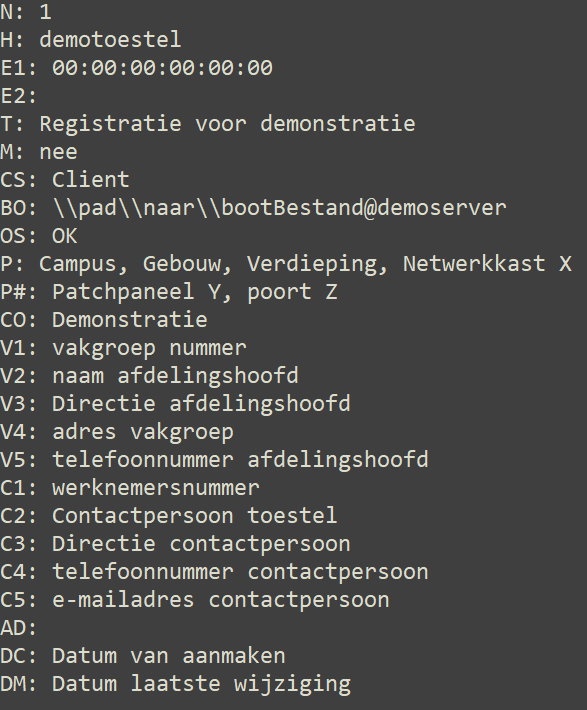
\includegraphics[height=0.4\textheight]{host.png}\label{fig:bezettehost}}
    \hspace*{\fill}
    \subfloat[Derde adres in het subnet is vrij om in te nemen]{%
        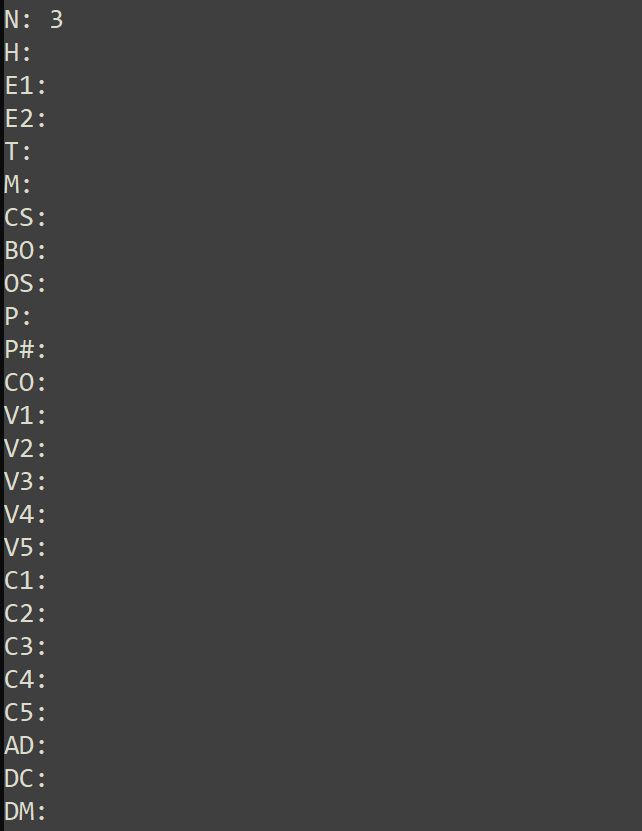
\includegraphics[height=0.4\textheight]{legeHost.png}\label{fig:legehost}}
    \caption{IP-reservatie en lege host entry in subnetbestanden}
    \label{fig:host}
\end{figure}

\subsection{Procedure IP registratie voor gebruikers}
Via de interne webpagina www.netadmin.ugent.be kunnen werknemers van UGent zowel nieuwe IP-reservaties aanvragen als bestaande IP-reservaties raadplegen, wijzigen of verwijderen. Bij een nieuwe aanvraag kan men naast de basisinfo ook de optionele parameters voor een host meegeven zoals beschreven in sectie \ref{subnetbestanden}. Bij wijzigingen kan men alle informatie van de registratie aanpassen, waardoor informatie aan de reservering kan worden toegevoegd, verwijderd of gewijzigd. Het verplaatsen van een host van een subnet naar een ander subnet is eveneens mogelijk door deze vraag mee te sturen naar de netwerkbeheerder via het opmerkingen-veld van de registratie. In figuur \ref{fig:netadmin} zijn de formulieren van deze website weergegeven met data voor demonstratiedoeleinden.

\clearpage
\begin{figure*}[h!]
    \centering
    \begin{subfigure}[b]{0.475\textwidth}
        \centering
        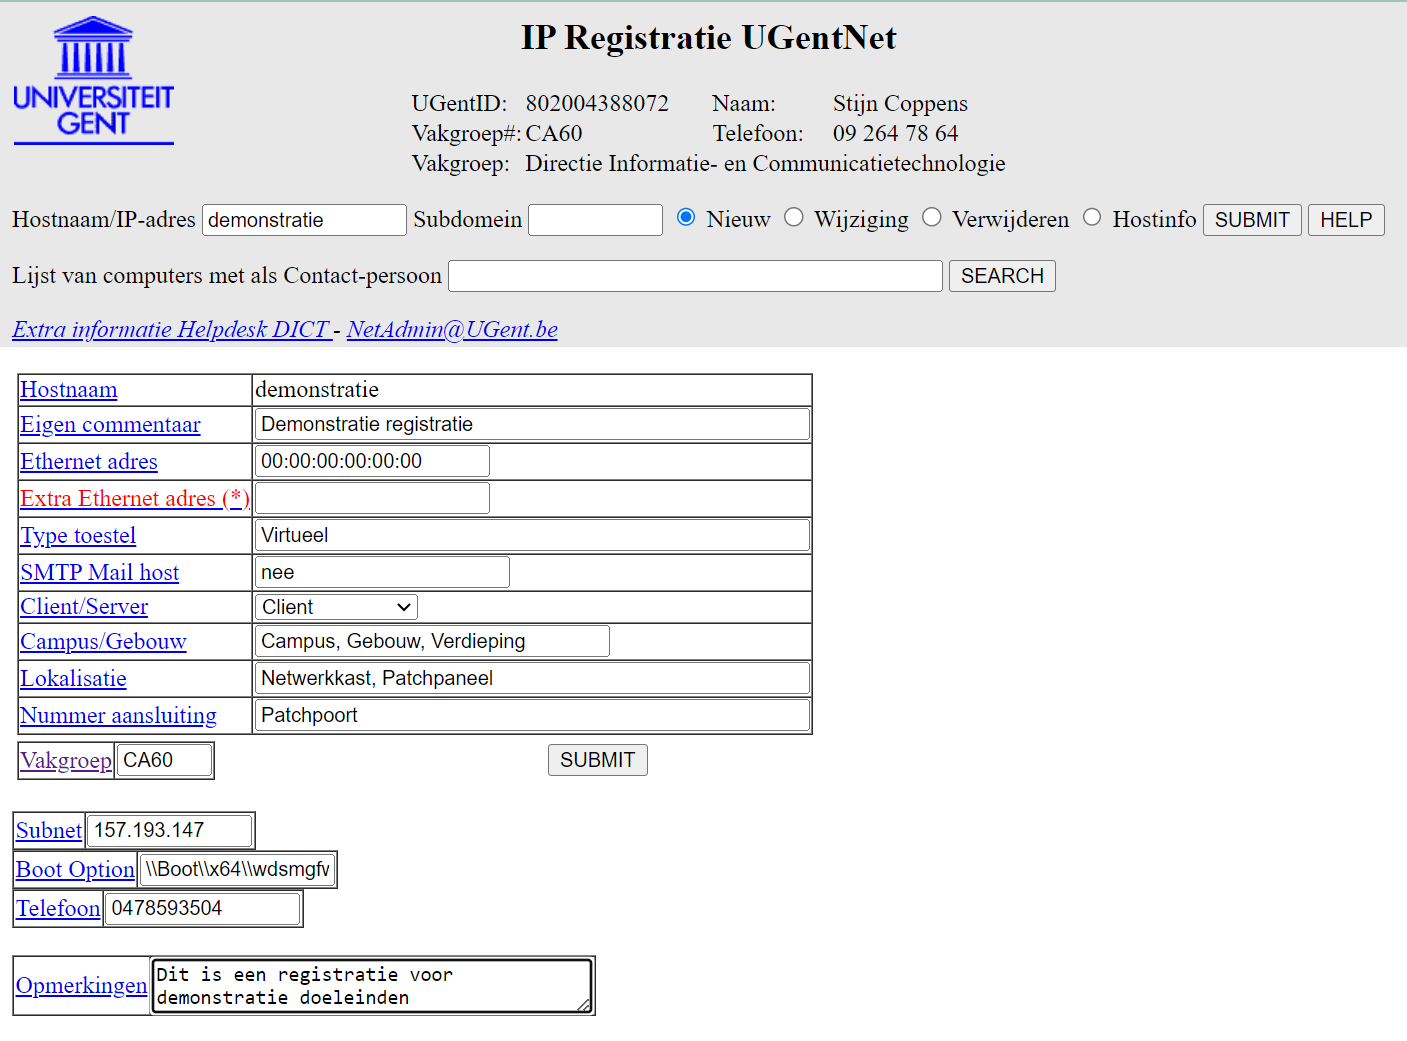
\includegraphics[width=\textwidth]{voorbeeldNieuweRegistratieNetadmin.png}
        \caption{Formulier nieuwe IP-registratie}
        \label{fig:formNieuwReg}
    \end{subfigure}%
    \hfill
    \begin{subfigure}[b]{0.475\textwidth}
        \centering
        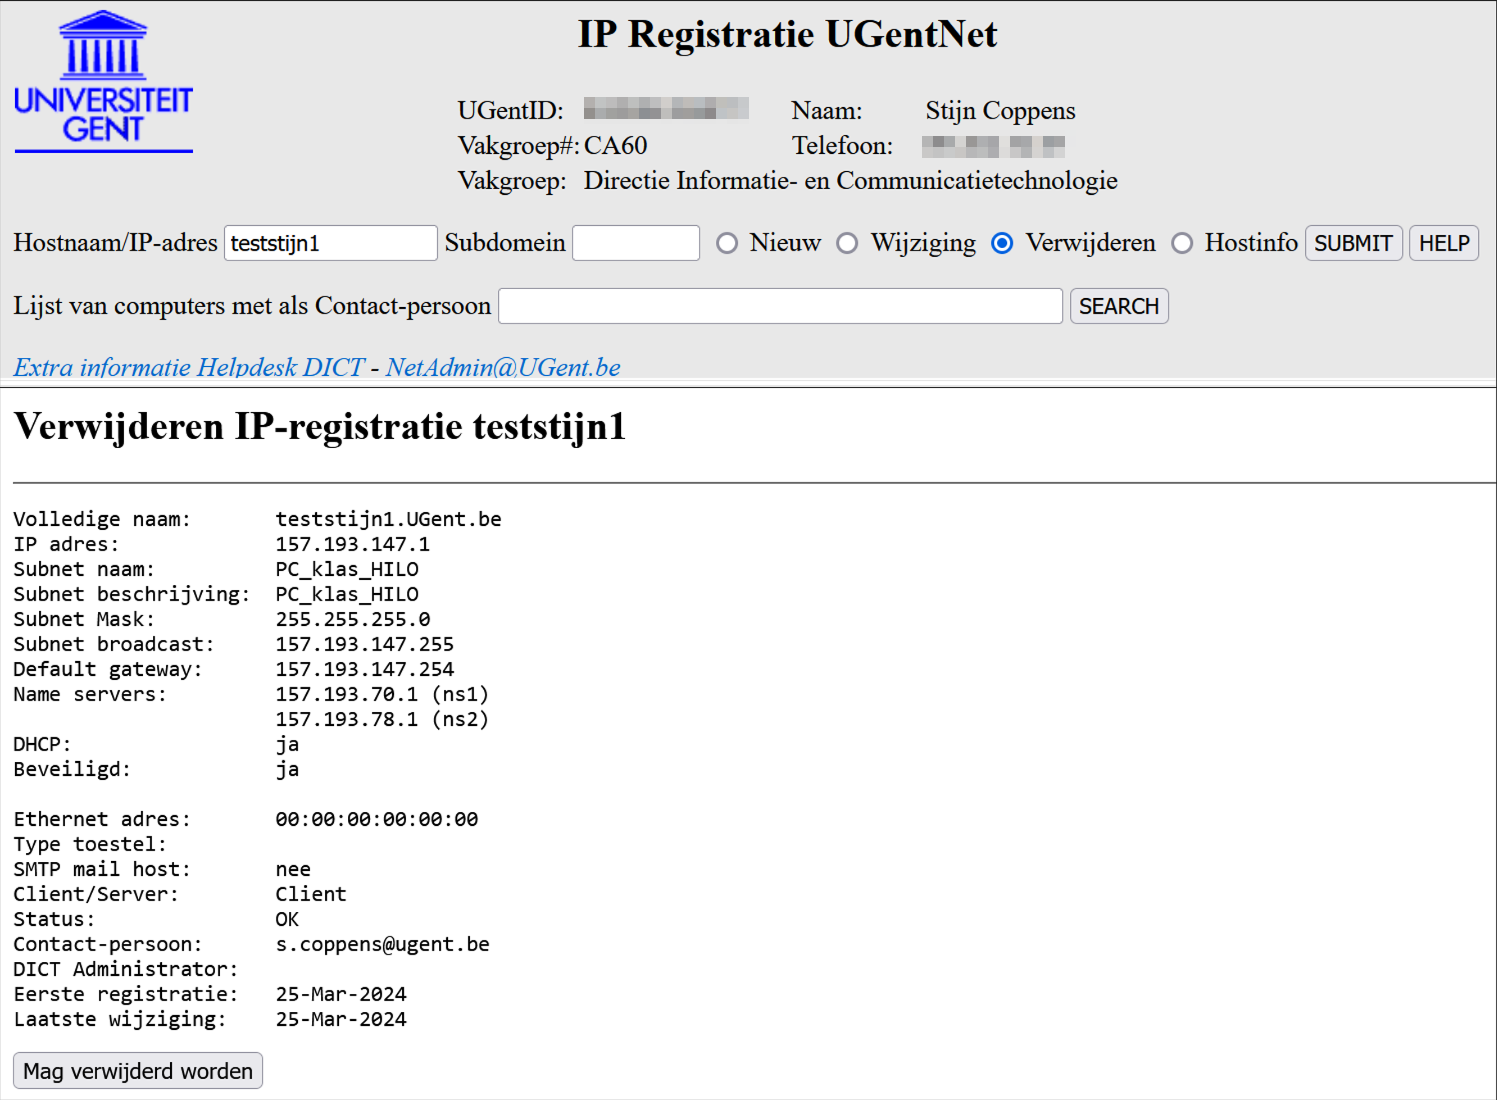
\includegraphics[width=\textwidth]{voorbeeldVerwijderingRegistratieNetadmin.png}
        \caption{Verwijdering IP-registratie}
        \label{fig:formVerwReg}
    \end{subfigure}
    \vskip\baselineskip
    \begin{subfigure}[b]{0.475\textwidth}
        \centering
        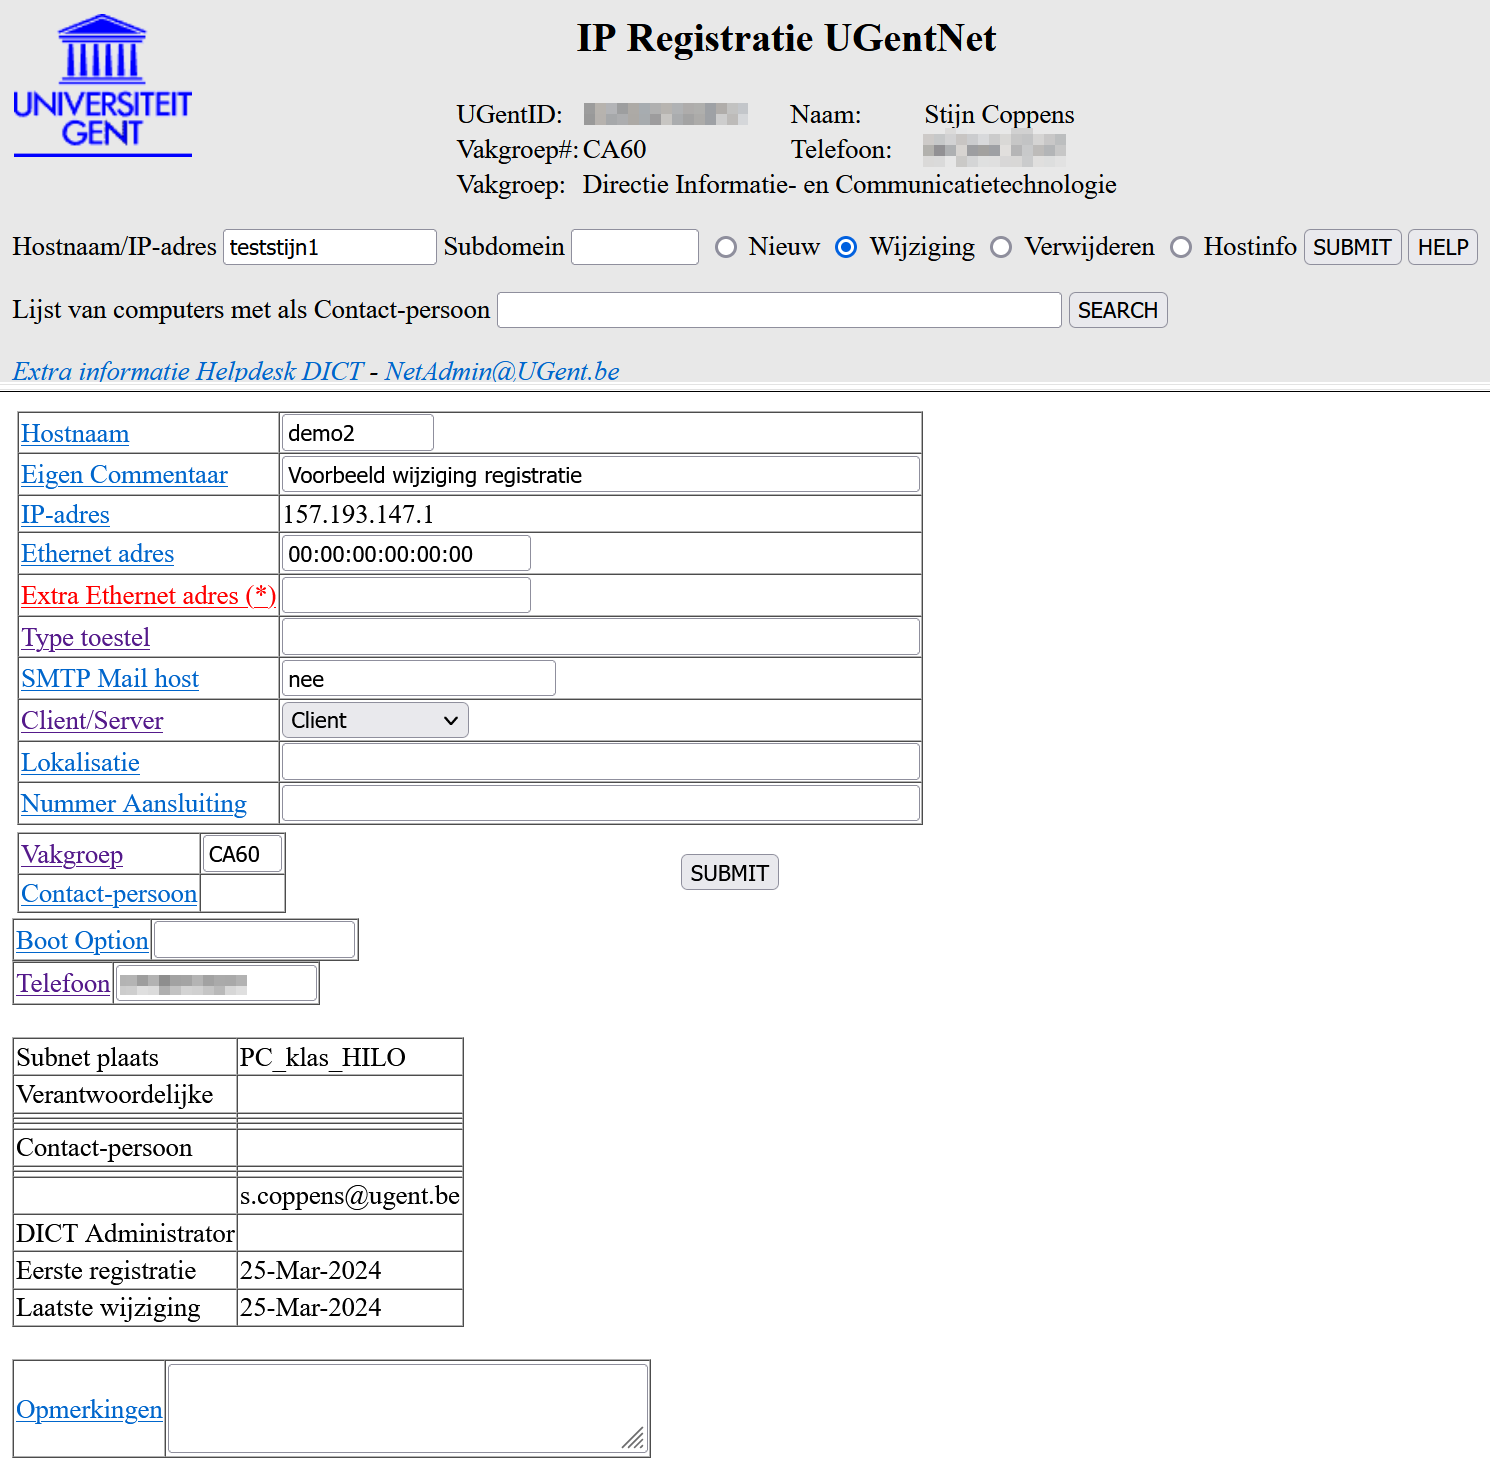
\includegraphics[width=\textwidth]{voorbeeldWijzigingRegistratieNetadmin.png}
        \caption{Formulier wijziging IP-registratie}
        \label{fig:formWijzReg}
    \end{subfigure}
    \hfill
    \begin{subfigure}[b]{0.475\textwidth}        
        \centering
        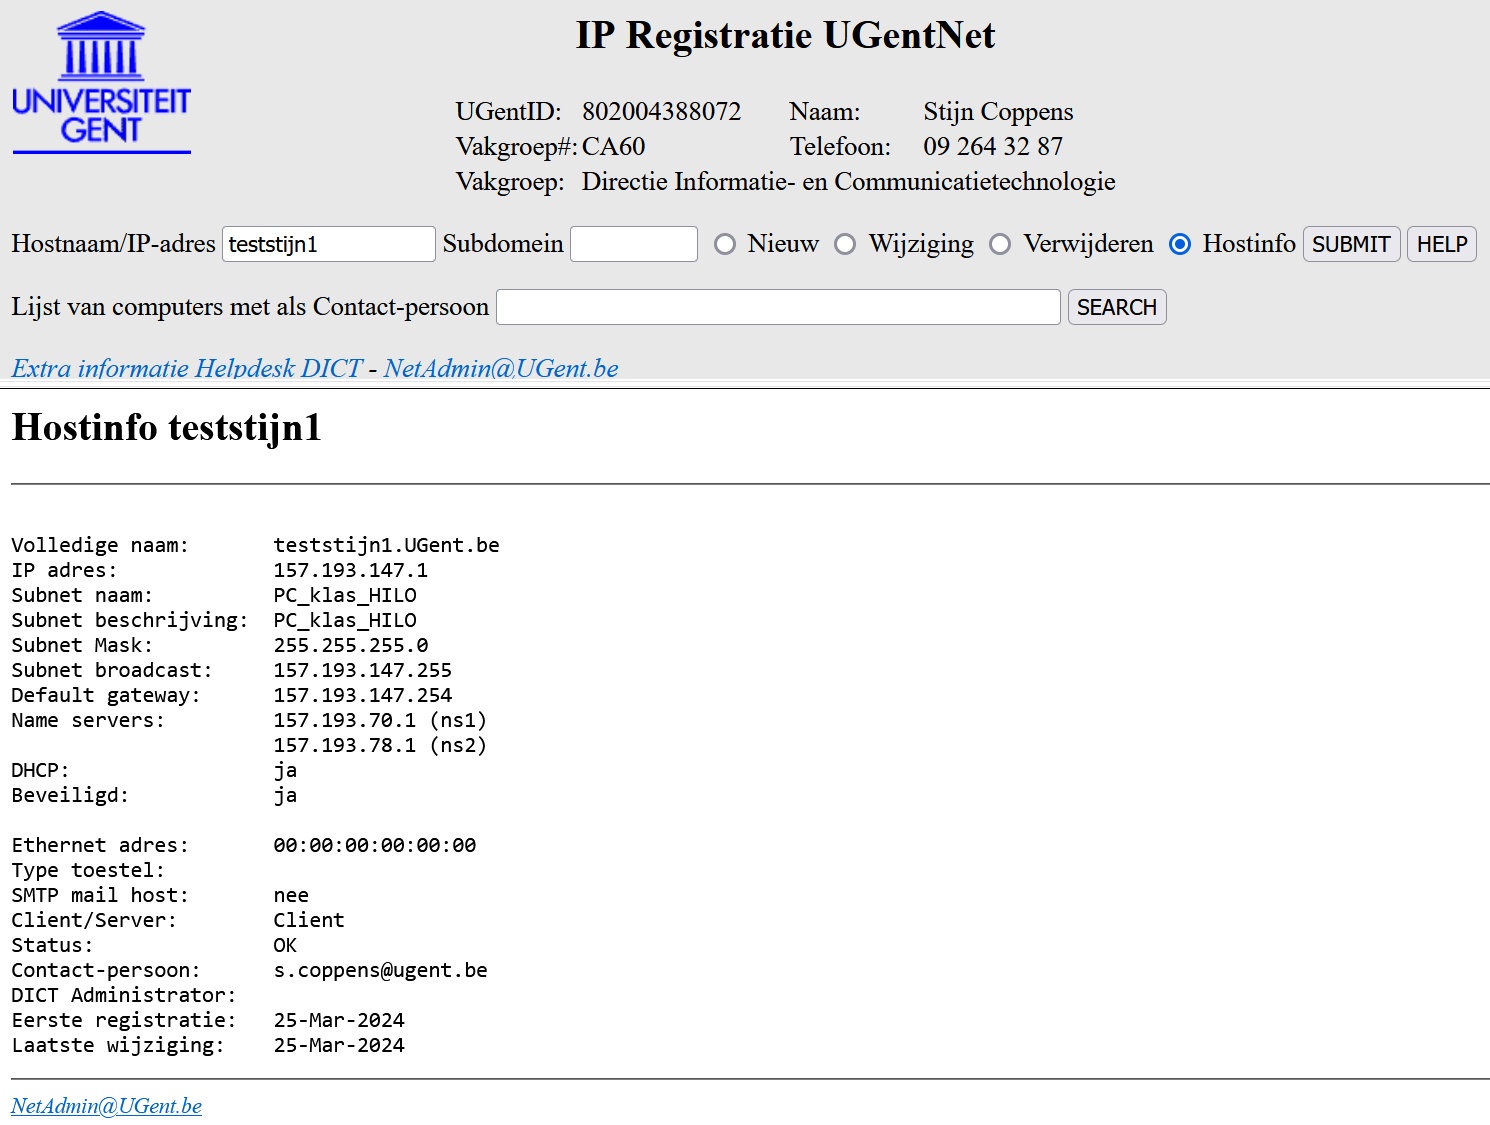
\includegraphics[width=\textwidth]{netadminRaadplegen.png}
        \caption{Raadplegen IP-registratie}
        \label{fig:raadReg}
    \end{subfigure}    
    \caption{Netadmin website IP-registratie}
    \label{fig:netadmin}
\end{figure*}


\subsection{Procedure IP registratie voor netwerkbeheerders}
Nadat de gebruiker op 'submit' klikt, zal de \textit{backend} van de website de ingegeven informatie verwerken en als mail verzenden naar de gedeelde mailbox 'netadmin@ugent.be'. Afbeelding \ref{fig:netadminMail} toont drie mails die een netwerkbeheerder dient te behandelen. Elke mail bevat een commando dat de netwerkbeheerder uitvoert op de daarvoor bestemde server in de folder waarin de subnetbestanden staan. Alle informatie in afbeeldingen \ref{fig:netadminMail} is gebaseerd op de gegevens die zijn ingevoerd in figuren \ref{fig:netadmin}.

\begin{itemize}
    \item \textbf{Figuur \ref{fig:nieuwRegMail}}: Deze mail geeft alle nodige informatie weer om een nieuwe IP-registratie te maken. Het in de mail beschreven commando \\\textbf{'mkh B 147 demotoestel'} zal enkele belangrijke taken en controles uitvoeren, waarna de cursor van de beheerder in het eerste vrije adres geplaatst wordt van subnetbestand subnetB147.000. Hierna kan de beheerder alles uit de mail kopiëren, beginnende bij \textit{21ddkA}, tot en met het einde van de host registratie. Nadat de beheerder het subnetbestand afsluit, zal het script nog enkele controles uitvoeren voor het geval er fouten in de registratie staan. Als de gebruiker in het opmerkingenveld nog informatie heeft geplaatst, zoals netwerkpoorten die open moeten staan, DNS Alias records of andere, dient de netwerkbeheerder dit manueel nog aan te vullen in het subnetbestand.
    \item \textbf{Figuur \ref{fig:wijzigRegMail}}: Deze mail bevat alles voor het wijzigen van een bestaande registratie, het commando in deze mail is \textbf{'chh B 147 teststijn1 demo2'}. Dit proces volgt een vergelijkbare uitvoering als bij het aanmaken van een nieuwe registratie. In dit geval wordt de opgegeven host \textit{teststijn1} gezocht in het subnetbestand subnetB147.000, waarbij de informatie in het subnetbestand wordt overschreven door die van de registratie. Omdat er een tweede hostnaam is opgegeven, zal het commando de hostnaam \textit{teststijn1} ook wijzigen naar de hostnaam \textit{demo2}.
    \item \textbf{Figuur \ref{fig:verwRegMail}}: Deze mail geeft het commando \textbf{'rmhost B 147 teststijn1'}. Dit commando zal, naast enkele controles voor \acrshort{acl}, de host in subnet B 147 opzoeken en vervangen door een lege, vrije host. Dit is het enige commando waarbij de netwerkbeheerder niet in het bestand hoeft te gaan om data te plaatsen, waardoor dit commando ook zeer beperkt is in uitvoeringstijd. Indien de host voorkomt in bepaalde ACL's kan het zijn dat de netwerkbeheerder eerst de relevante 'S'-lijnen bij andere hosts zal moeten verwijderen waarin deze host voorkomt.
\end{itemize}

\begin{figure}[H]
    \subfloat[Nieuwe IP-registratie]{%
        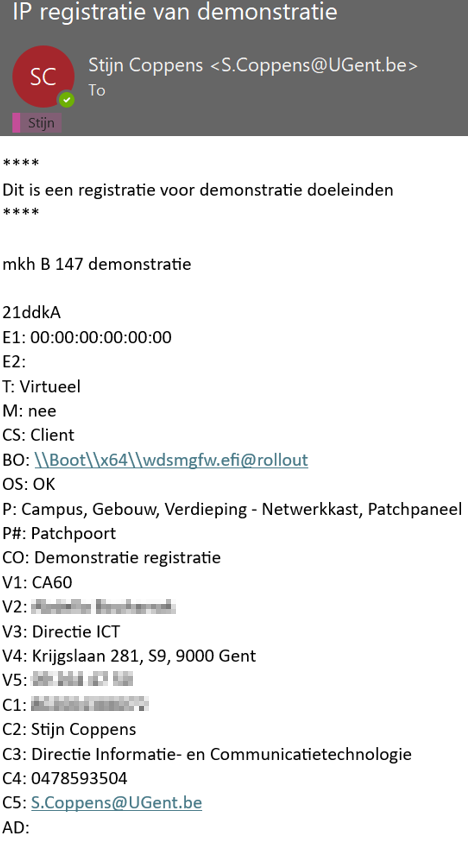
\includegraphics[height=0.4\textheight]{mailNieuweRegistratie.png}
        \label{fig:nieuwRegMail}}
    \hspace*{\fill}
    \subfloat[Wijziging hostnaam IP-registratie]{%
        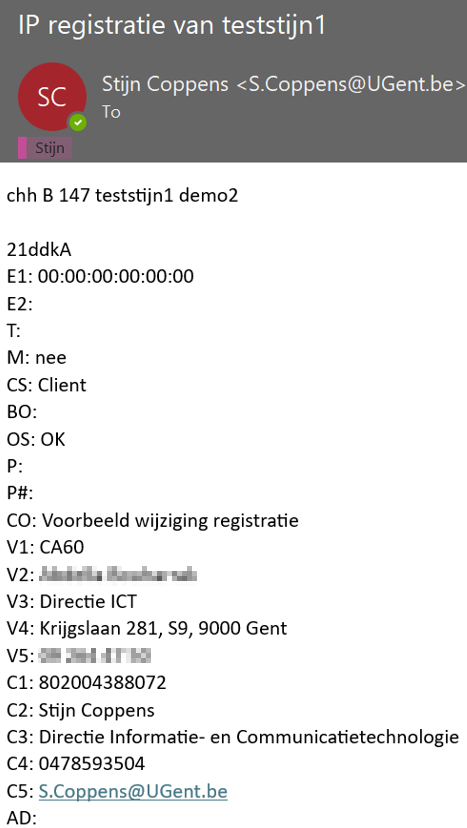
\includegraphics[height=0.4\textheight]{mailWijzigingRegistratie.png}
        \label{fig:wijzigRegMail}}
    \hspace*{\fill}
    \subfloat[Verwijderen IP-registratie]{%
        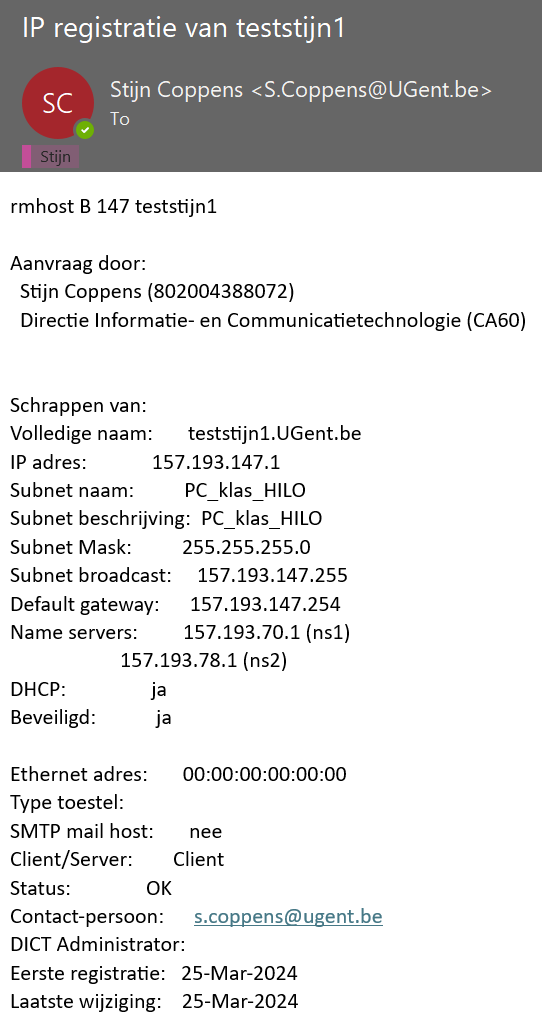
\includegraphics[height=0.4\textheight]{mailVerwijderenRegistratie.png}
        \label{fig:verwRegMail}}
    \caption{Mails IP-Registratie}
    \label{fig:netadminMail}
\end{figure}

\subsection{Aanvullende belangrijke commando's voor subnetbestanden}
Naast de drie commando's \textbf{'mkh'}, \textbf{'cch'} en \textbf{'rmhost'} voor het verwerken van IP-registraties, zijn er nog enkele andere commando's die relevant zijn:

\begin{itemize}
    \item \textbf{Hosts verplaatsen}: vb. \textbf{'mvh B 147 B 50 teststijn1'} zal een host verplaatsen van subnetbestand subnetB147.000 naar subnetB050.000.
    \item \textbf{Subnetten opschonen}: vb. \textbf{'unused B 147 400'} geeft alle hosts weer die 400 dagen offline zijn, \textbf{'unused\_rmhost B 147 400'} geeft alle commando's om diezelfde hosts te verwijderen. Om dit werkende te krijgen worden de \acrshort{arp}-tabellen van alle routers binnen UGent meerdere keren per dag uitgelezen. Wanneer een apparaat verbinding maakt met het netwerk, wordt het \acrfull{mac}-adres, een uniek adres dat door de fabrikant van het apparaat is toegewezen, altijd opgenomen in deze tabel. Als het MAC-adres van een host uit subnet B147 bijvoorbeeld gedurende 400 dagen niet is verschenen in de betreffende ARP-tabel voor zijn IP-adres, wordt het met dit commando weergegeven. Subnetten worden opgekuist als de netwerkbeheerder een melding krijgt bij het maken van een nieuwe registratie dat het subnet vol is.
\end{itemize}

Naast deze commando's zijn er ook nog de update-commando's. Pas nadat deze uitgevoerd zijn, zullen alle registraties die gemaakt zijn sinds de vorige uitvoering ook effectief van toepassing zijn. De update-commando's zijn:

\begin{itemize}
    \item \textbf{'update\_all -load'}: Dit commando zal alle nodige DNS-bestanden aanmaken en actief zetten in de DNS-server.
    \item \textbf{'update\_dhcp'}: Dit commando zorgt ervoor dat alle aanpassingen voor DHCP toegepast worden op de DHCP-server.
    \item \textbf{'update\_hostlst'}: Dit commando zorgt ervoor dat de hostinfo beschikbaar is voor gebruikers op o.a. de netadmin registratie website.
    \item \textbf{'mkacl'}: Dit commando overloopt alle aangemaakte ACL's en genereert de nodige configuratiebestanden voor de routers.
    \item \textbf{'update\_acl\_write'}: Dit commando zal bij de start van het uitvoeren een wachtwoord opvragen aan de netwerkbeheerder die dit commando ingeeft. Via dit wachtwoord zal dit commando alle ACL-aanpassingen communiceren met de nodige routers.
\end{itemize}

%\begin{figure}[H]
%    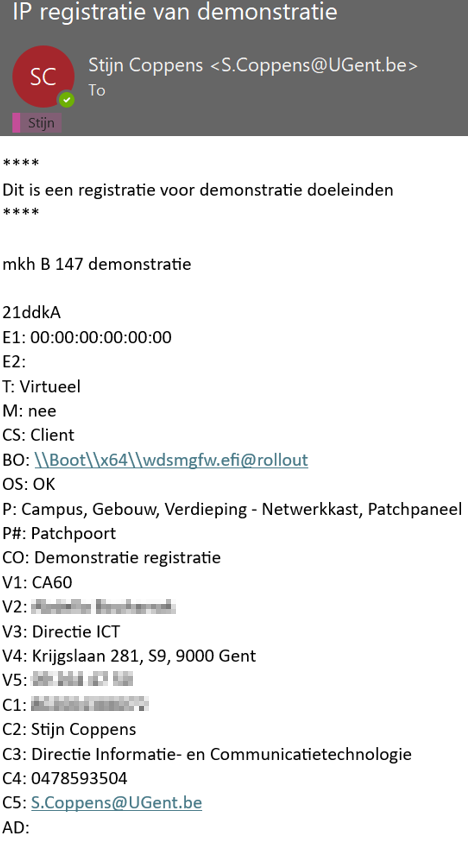
\includegraphics[height=7cm]{mailNieuweRegistratie.png}
%    \caption{Inhoud mail van nieuwe IP-registratie}
%    \label{fig:netadminMail}
%\end{figure}

\subsection{Evaluatie subnetbestanden}
\label{uitdagingen}
Het gebruiken van deze subnetbestanden brengt meerdere uitdagingen met zich mee:
\begin{itemize}
    \item \textbf{Tijd}: Het manueel onderhouden van de scripts, subnetbestanden, netwerkadresreservaties (maken en opschonen) kan veel tijd vragen. Alle mails met IP registraties moeten elk afzonderlijk bekeken en verwerkt worden.
    \item \textbf{Schaalbaarheid}: Doordat elke wijziging het bestaande bestand overschrijft en er dus geen historische data is, kan men moeilijk trends herkennen. Ook wikipagina's moet men manueel bijwerken bij grote wijzigingen in de structuur. Daarnaast zijn deze tekstbestanden gericht op IPv4 en is deze methode niet bruikbaar om IPv6 te implementeren aangezien IPv6 een veel groter bereik heeft en een andere notatie gebruikt.
    \item \textbf{Consistentie}: De huidige aanpak vraagt meerdere manuele acties, waardoor die vatbaar is voor menselijke fouten of vergissingen. Ook het manueel opzoeken van de relevante subnetbestanden als de aanvrager niet weet in welk subnet de aanvraag terecht moet komen, kan leiden tot registraties in verkeerde subnetten.  
    \item \textbf{Beveiliging}: Zoals beschreven door \textcite{Liao2020} is een van de eerste stappen in een cyberaanval het verzamelen van netwerk informatie via netwerk scan tools zoals 'Nmap'. Omdat alle IP-registraties van het volledige domein centraal in ongecrypteerde bestanden worden opgeslagen, zijn deze leesbaar voor iedereen die toegang heeft tot de bestanden. Deze bestanden vormen dus een schat aan informatie voor elk individu, ongeacht of hun bedoelingen goed of slecht zijn. Daarnaast kan ook niet worden nagekeken wie wanneer welke registratie heeft aangemaakt, wat onveilig kan zijn omdat er geen controle en verantwoordelijkheid is over de wijzigingen. Zonder deze informatie is het onmogelijk om wijzigingen te auditen, fouten te traceren, of ongeautoriseerde wijzigingen op te sporen, wat kan leiden tot beveiligingsrisico's en operationele problemen in het netwerkbeheer.
\end{itemize}


\section{Status migratie subnetbestanden naar EfficientIP}
\label{premigratie}
Eind 2023 werden de eerste stappen genomen in het project om EfficientIP te implementeren in de werking. Dit project wordt uitgevoerd door Mevr. A. Vandermeeren, vanwege haar uitgebreide kennis van DNS en DHCP binnen UGent en Dhr. S. Coppens die de nodige scripts schrijft.
Dit project maakt gebruik van volgende testen, deze worden uitgevoerd zowel bij het implementeren van nieuwe functionaliteiten als bij het testen van scripts:
\begin{itemize}
    \item \textbf{Manuele EfficientIP testen}: Om na te gaan hoe EfficientIP werkt en hoe bepaalde functionaliteiten reageren op nieuwe informatie worden manuele testen gedaan via de webinterface van EfficientIP.
    \item \textbf{Postman API-testen}: Via het programma Postman worden manuele testen geschreven die via HTTPS verstuurd worden naar EfficientIP. Dankzij deze testen is er meer inzicht hoe EfficientIP reageert en welke informatie noodzakelijk is.
    \item \textbf{Host- en subnettesten}: Om meerdere scenario's te controleren worden in subnetbestand 'subnetB147.000' testen gedaan met het aanmaken, wijzigen en verwijderen van hosts.
\end{itemize}
Sinds het begin van het project zijn de volgende drie Python-scripts geschreven. Elk van deze scripts draait apart op Nomad. Dit is een systeem dat ervoor zorgt dat de scripts betrouwbaar en flexibel worden uitgevoerd in een virtuele omgeving, wat bijdraagt aan een stabiele en efficiënte werking.
\begin{itemize}
    \item \textbf{UploadSubnetFile}: Dit script maakt via \acrshort{ssh} en \acrshort{scp} een veilige verbinding met de server waarop de subnetbestanden staan en maakt van al deze bestanden een kopie in de virtuele omgeving waarin het script draait. Hierna doorloopt het script elk bestand, waarop die voor elk bestand de nodige API-oproepen doet om subnetwerken en hosts aan te maken op EfficientIP.
    \item \textbf{CreateSubnetFile}: Dit script stuurt een API-oproep naar EfficientIP om alle subnetten op te halen. Hierna haalt het script opnieuw via een API-oproep voor elk subnet alle hostadressen op. Daarna zal het script, in de virtuele omgeving waarin die draait, voor elk subnet de nodige subnetbestanden aanmaken. Eens al deze subnetbestanden zijn aangemaakt, haalt dit script een kopie op van de productie-subnetbestanden, waarop het script voor elk bestand een log wegschrijft met de verschillen tussen het nieuw aangemaakte bestand en het productie-bestand. Tenslotte maakt het script gebruik van SSH en SCP om een veilige verbinding te maken met de server waarop de productie-subnetbestanden zijn opgeslagen. Het script plaatst de nieuwe subnetbestanden in een tijdelijke map op deze server voor later nazicht en uploadt ook alle logbestanden naar de map voor de logs.
    \item \textbf{CompareAndUpdate}: Omdat een referentiepunt nodig is om de aanpassing\-en te ontdekken in de productie-subnetbestanden, werd op dezelfde server de folder 'LastState' aangemaakt. In deze folder wordt bij elke succesvolle uitvoering van het script een kopie geplaatst van al de productie-subnetbestan\-den. Dit script start met via SSH en SCP een veilige verbinding op te zetten met de server waarop de subnetbestanden staan, om daar dan de datum op te halen van een subnetbestand in de 'LastState'-folder. Hierna zal het script de laatst bewerkte datum van alle productie-subnetbestanden overlopen. Voor elk productie-subnetbestand dat een nieuwere datum heeft, wordt een kopie overgezet van zowel het productie-subnetbestand als de versie in de 'LastState'-folder naar de virtuele omgeving waarin het script draait. Hierna worden alle verschillen overlopen tussen de twee versies en worden de nodige API-oproepen gedaan om EfficientIP te updaten. Als alle API-oproepen een succesvol antwoord gekregen hebben, zal het script tenslotte een kopie maken van al de huidige productie-subnetbestanden naar de 'LastState'-folder op de productieserver. Indien er fouten voorkomen tijdens het uitvoeren van het script, blijft de 'LastState'-folder ongewijzigd en zal de oorzaak voor de fouten terug te vinden zijn in de logs van de virtuele omgeving waarin het script draait.
\end{itemize}

\section{Volgende stappen in de migratie}
Eens de testen geslaagd zijn voor de drie scripts uit sectie \ref{premigratie} zal het mogelijk zijn om EfficientIP synchroon mee te laten draaien naast de productie-omgeving. Eens dit in orde is, is het mogelijk om de website te implementeren van waaruit registraties gemaakt kunnen worden die naar EfficientIP gaan. Hoe de implementatie van de website zal gebeuren, is terug te vinden in het volgende hoofdstuk \ref{ch:methodologie}.


